% ---------------------------------------------------
%
% Trabajo de Fin de Grado. 
% Author: Alejandro Hernández Padrón. 
% Capítulo: La aplicacion ULL-Navigation. 
% Fichero: Cap4_TheApplication.tex
%
% ----------------------------------------------------
%

\chapter{La aplicación ULL-Navigation} \label{chap:LaAplicacion} 

En este capítulo explicaremos la aplicación ULL-Navigation utilizando la especificación de requisitos de la misma y explicando su funcionamiento.

\section{Especificación de requisitos} % (fold)

Nos dispondremos a exponer los requisitos de la presente aplicación propuesta para el desarrollo de este TFG.

Se trata de una aplicación móviles, más concretamente a aquellos dispositivos que utilizan Android como sistema operativo. Es una aplicación diseñada para los estudiantes de la Universidad de La Laguna (ULL) la cual les permita ubicarse, detectar y reconocer los centros y edificios pertenecientes a la universidad mediante técnicas de Realidad Aumentada basadas en la geolocalización.

Los requisitos principales de la aplicación son:
\begin{itemize}
    \item La aplicación se desarrollará para dispositivos con Android. Se utilizará Android Studio como entorno de desarrollo integrado(IDE) para su desarrollo.
    \item Se implementarán técnicas de Realidad Aumentada basadas en la geolocalización para mostrar al usuario el centro universitario al cuál apunta con la cámara.
    \item Los centros de la Universidad de La Laguna junto a su información correspondiente estarán ubicadas en un base datos en la nube y a su vez el servidor que se comunique con esta deberá estar en la nube.
\end{itemize}


\section{Especificación detallada de los requisitos} 

A continuación se expondrán de forma más detallada cada uno de los requisitos de la aplicación.

La aplicación se iniciará una Splash Screen\cite{URL::SplashScreen} o pantalla de inicio con el logo de la Universidad de La Laguna. Esta pantalla dará paso a una ventana de login.

Para poder utilizar la aplicación el usuario a ser alumno de la Universidad de La Laguna y poseer su respectiva cuenta de Google con el correo institucional de la universidad con el formato ``\textit{aluxxxxxxxxxx@ull.edu.es}''. Sin ella no se podrá acceder a la aplicación. Además se podrá cerrar la sesión de esta cuenta.

Una vez logueado accederemos a venta de inicio en la que aparecerá un acceso directo a las ventanas de \textit{Mapa ULL} y \textit{Navegación en modo RA} que explicaremos más adelante. Además dispondrá de los accesos directos a enlaces de interés de Universidad de La Laguna que se abrirán en un navegador externo.

Una vez dentro de la aplicación tendremos menú para movernos por las diferentes ventanas. Se utilizará un menú deslizante lateral o \textit{Navigation Drawer}\cite{URL::NavigationDraw} ubicado en la parte superior izquierda de la aplicación. Este menú deberá ser simple e intuitivo.

Como accesos en este menú disponemos de las siguientes ventanas:

\begin{itemize}
    \item Mapa ULL: Esta ventana contendrá un mapa de la universidad con todos los centros en la base de datos. 
    \item Navegación en modo RA: En esta ventana mediante el uso de la cámara se identificarán los centros universitarios a los que esta apunte y permitirá mostrar una pestaña con información detallada del los mismos.
    \item Centros de la ULL: Contiene todas la ubicaciones y centros de la Universidad de La Laguna y permitirá la búsqueda de los mismos. 
    \item Configuración: Permitirá acceder a los ajustes de la aplicación.
    \item Cerrar cesión: Cerrará la sesión actual y nos devolverá a la ventana de login
    \item Info: Información de aplicación así como su autor.
\end{itemize}

Cada centro de la universidad tendrá una ficha de información que será accesible desde una ventana de la aplicación con la siguiente información:

\begin{itemize}
    \item \textbf{Id}: Con él identificaremos el centro.
    \item \textbf{Nombre}: Nombre oficial del centro
    \item \textbf{Ubicación}: La ubicación exacta en la que se encuentra el centro. 
    \item \textbf{Descripción}: Descripción del centro con el objetivo y actividades que se desarrollan en él.
    \item \textbf{Imagen}: Imagen del centro.
    \item \textbf{Lista de enlaces de interés}: Una lista con los enlaces a las instituciones, servicios, departamentos y grados que se imparten en este centro.
\end{itemize}

Esta información estará guardada en una base de datos en la nube. Para acceder a está se dispondrá de un servidor en la nube que conecte con la base de datos y envié la información a la aplicación.

\section{Ventanas de la aplicación}


Nada más iniciar la aplicación nos encontramos con dos ventanas:

\begin{figure}[h]
\hspace*{\fill}%
\begin{subfigure}[h]{0.35\linewidth}

\includegraphics[width=\linewidth]{splashApp}
\caption{Splash-Screen.}
\label{fig:splashApp}
\end{subfigure}
\hfill%
\begin{subfigure}[h]{0.35\linewidth}
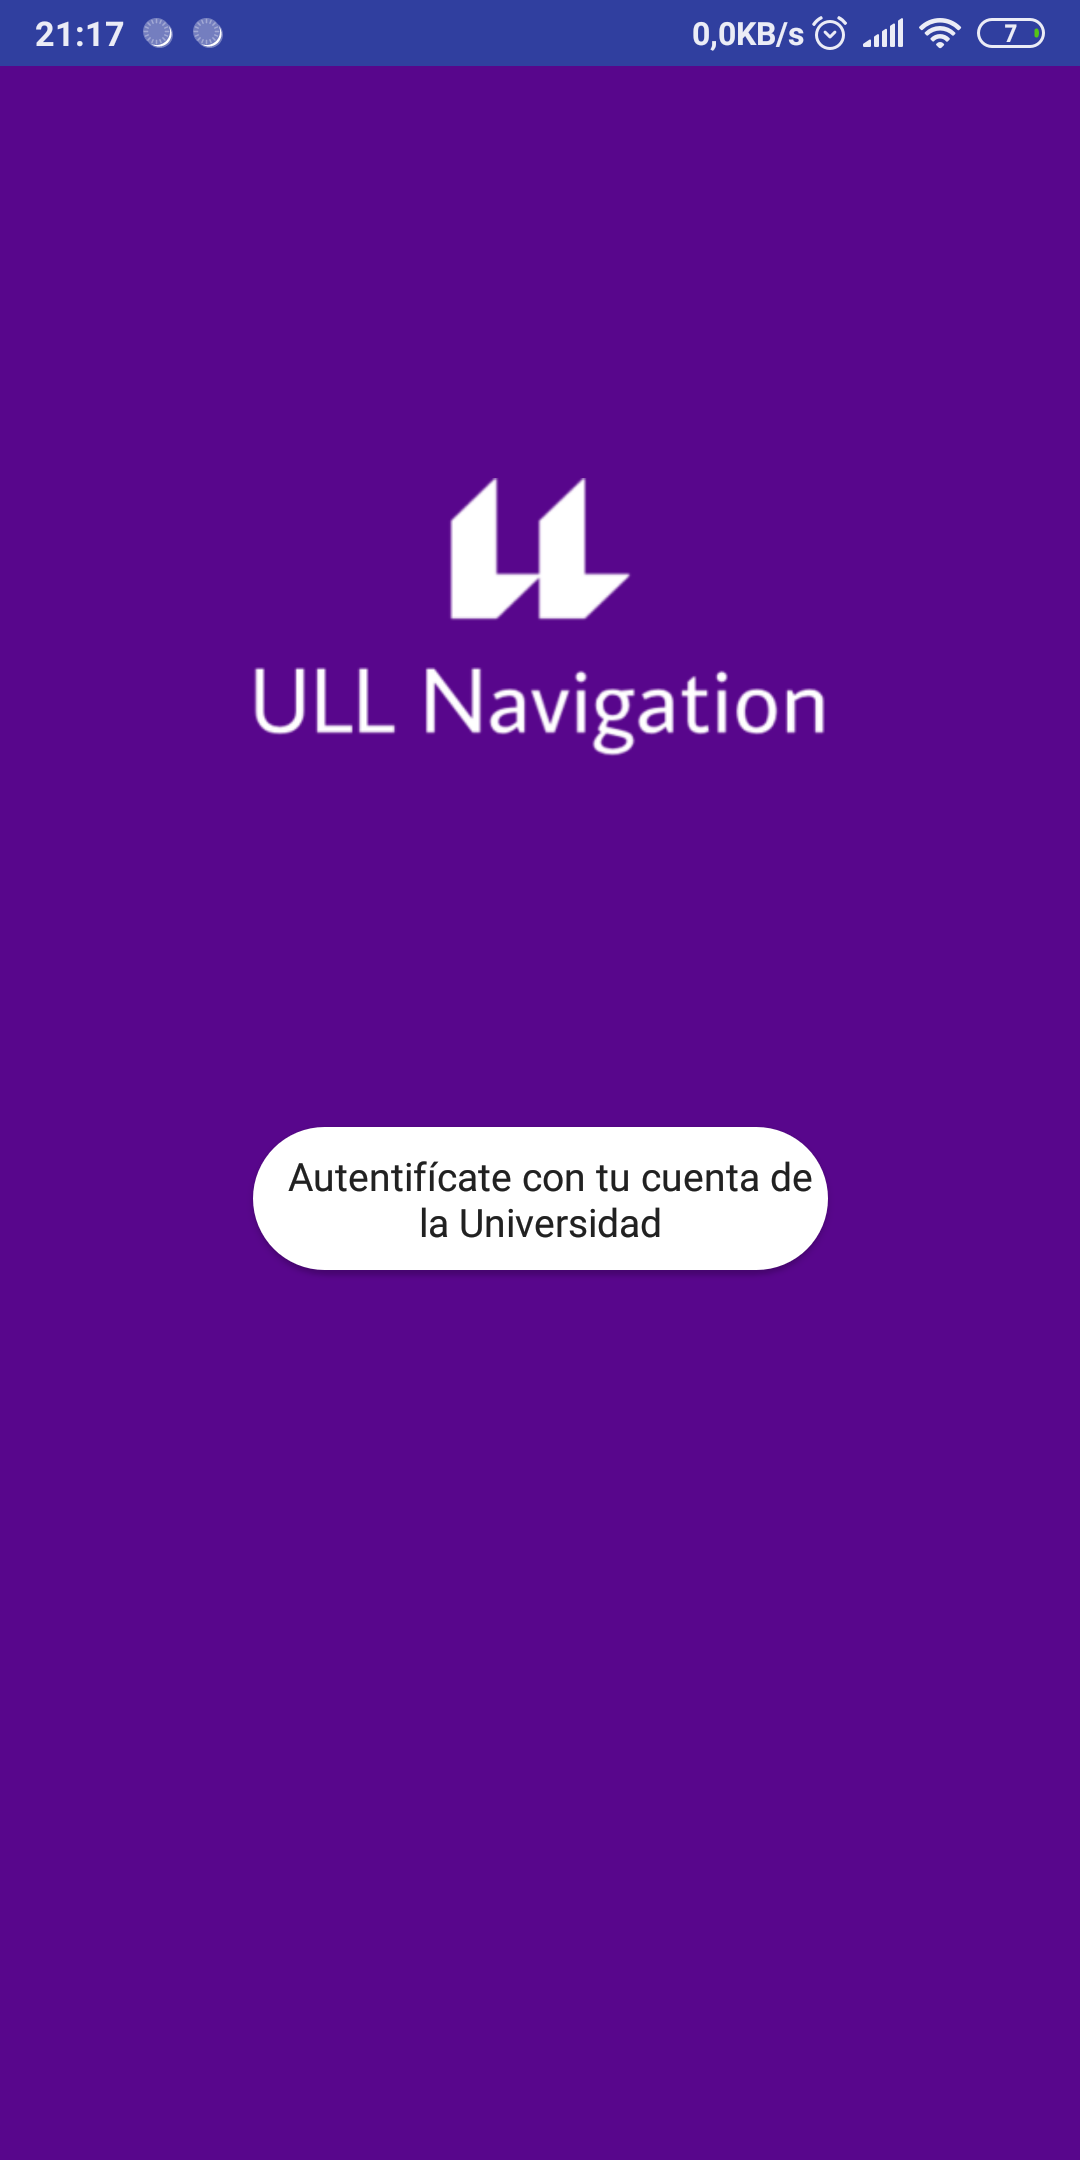
\includegraphics[width=\linewidth]{loginApp}
\caption{Login.}
\label{fig:loginApp} 
\end{subfigure}%
\caption{Ventanas de iniciales de \textit{ULL-Navigation}.}
\hspace*{\fill}%
\end{figure}
  
La primera imagen (vease Figura \ref{fig:splashApp}) es la pantalla de inicio que se aparece cuando ejecutamos la aplicación. Tras unos segundos, se carga la ventana del login(vease Figura \ref{fig:loginApp}). En esta tendremos que tener una cuenta de Google de la ULL. Una vez pinchamos en el botón del medio se nos abre una ventana de diálogo para que pongamos nuestra cuenta.

Cuando nos hayamos logueado con éxito se nos abrirá la venta de \textit{Inicio} (vease Figura \ref{fig:homeApp}) en la que tendremos una lista de accesos directos a las funcionalidad principales de la aplicación, como són \textit{Navegación en modo RA}, \textit{Mapa ULL} y enlaces a sitios web de la ULL.


\begin{figure}[h]
    \hspace*{\fill}%
    \begin{subfigure}[h]{0.35\linewidth}
    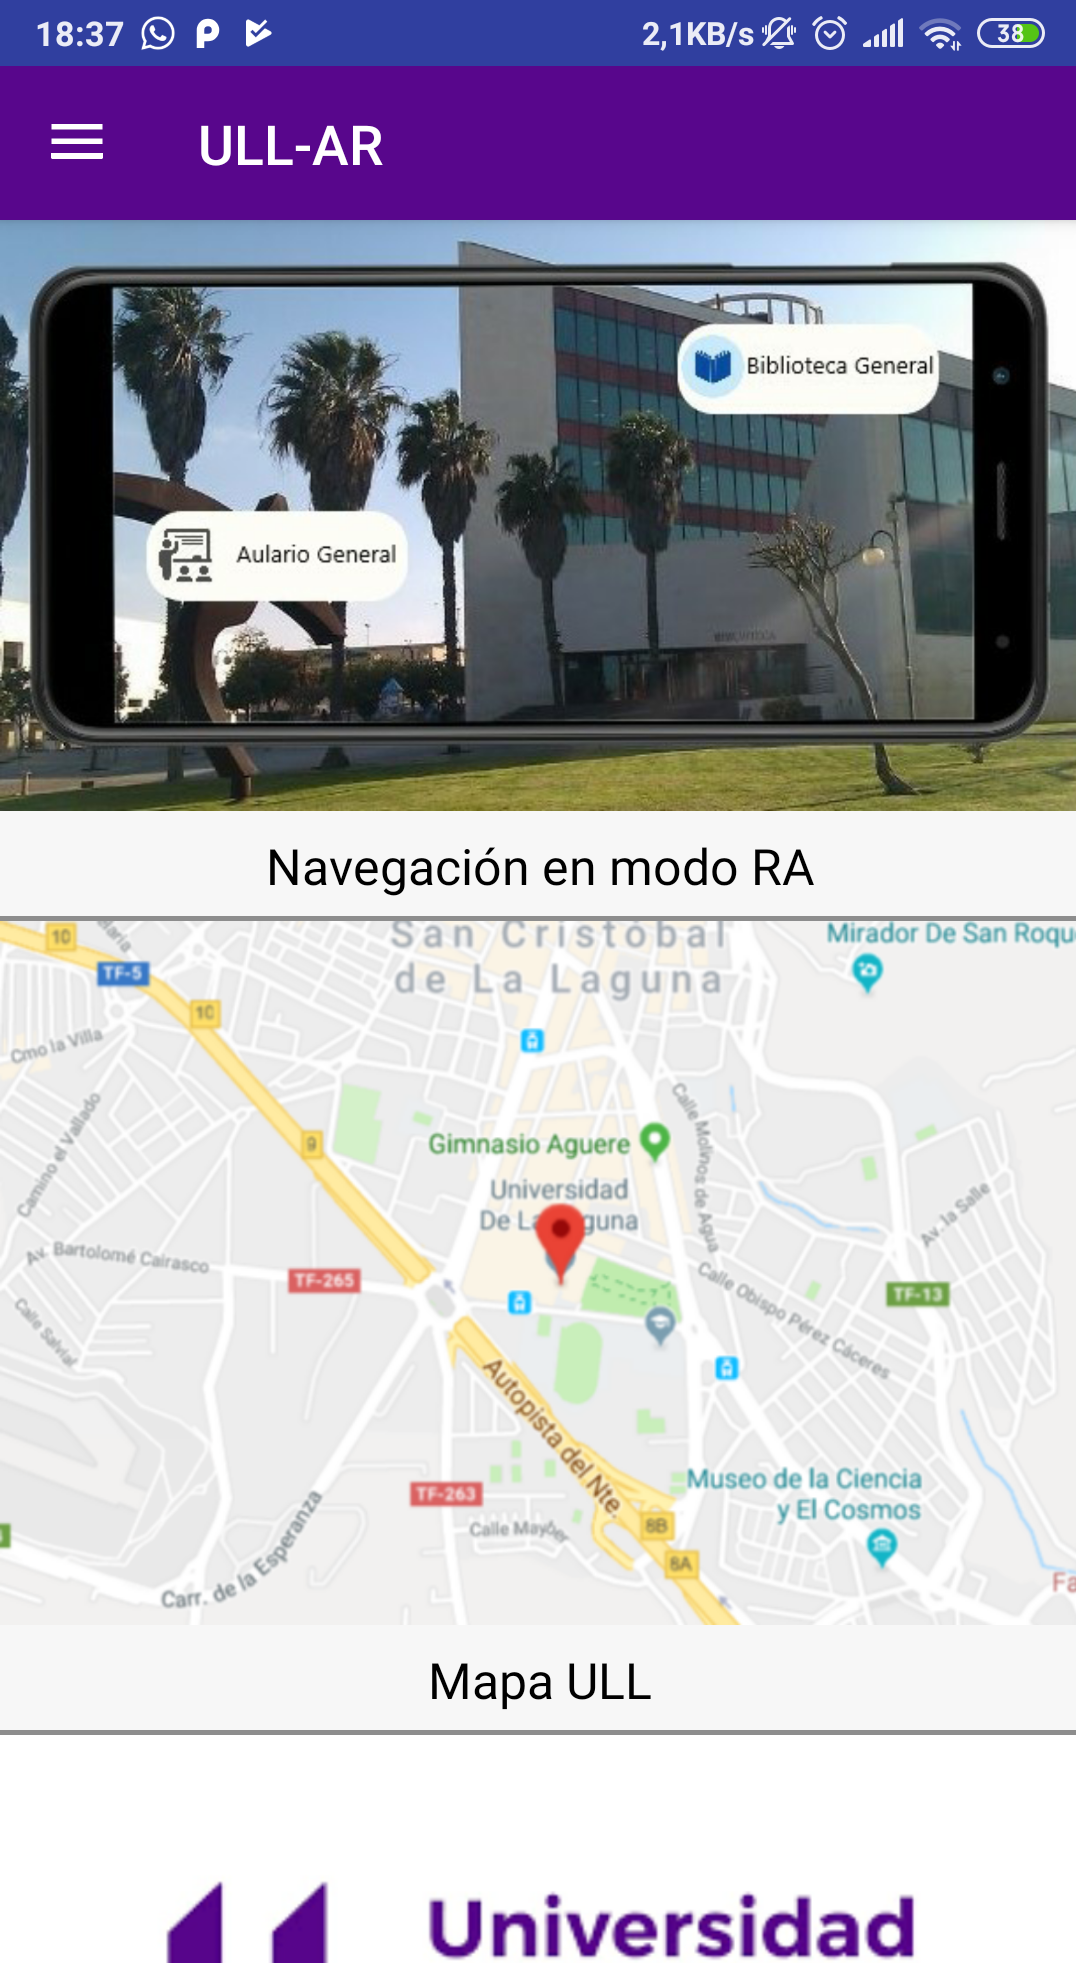
\includegraphics[width=\linewidth]{homeApp}
    \caption{Inicio.}
    \label{fig:homeApp}
    \end{subfigure}
    \hfill%
    \begin{subfigure}[h]{0.35\linewidth}
    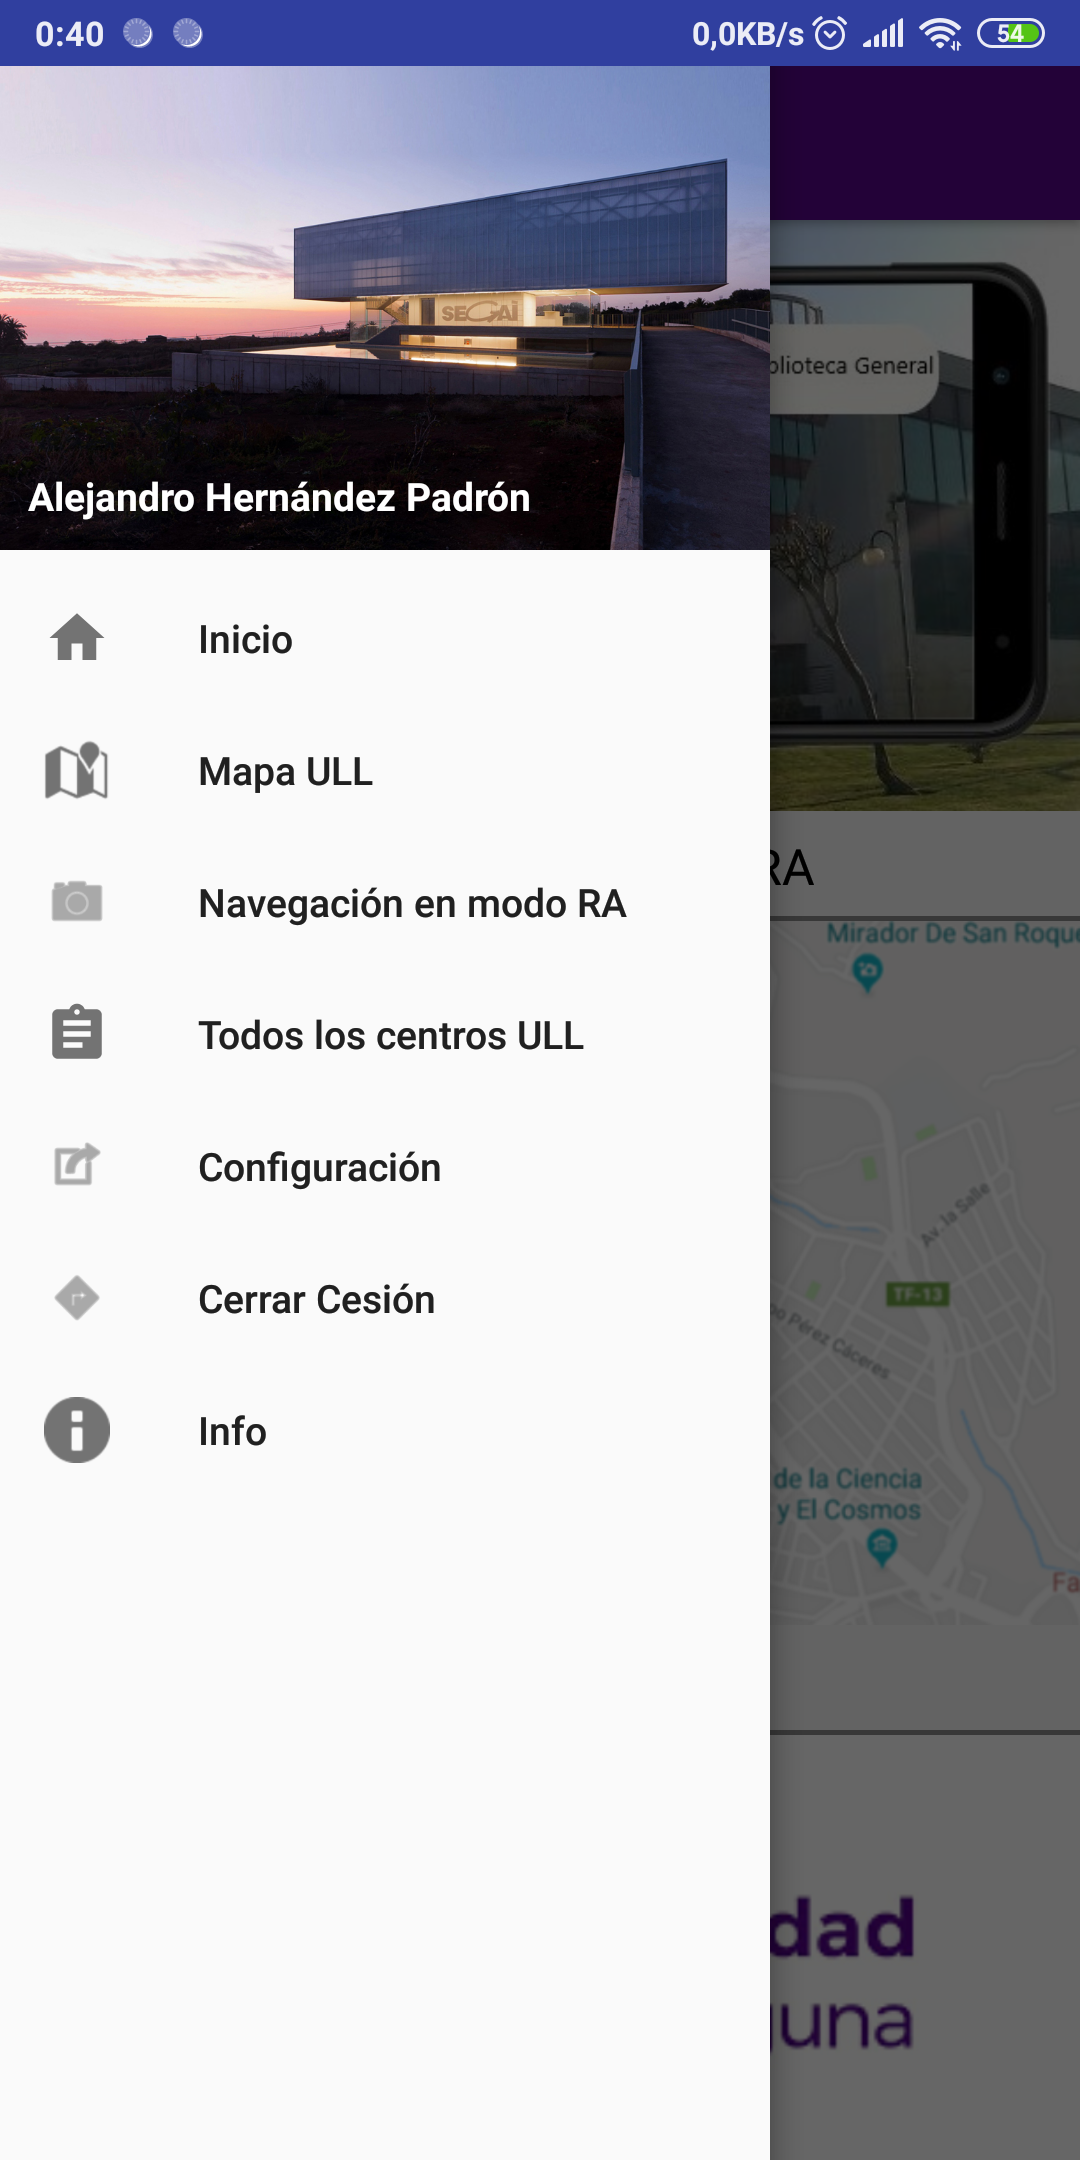
\includegraphics[width=\linewidth]{menuApp}
    \caption{Menu. Navigation Drawer.}
    \label{fig:menuApp}
    \end{subfigure}%
    \caption{Ventana \textit{Inicio} y el \textit{Menú} de \textit{ULL-Navigation}.}
    \hspace*{\fill}%
\end{figure}


En la esquina superior izquierda de aplicación tenemos el acceso al menú \textit{Navigation Drawer}. Si lo pulsamos se nos desplegará el menú que nos permite movernos por las distintas ventanas de la aplicación (vease Figura \ref{fig:menuApp}).

Si nos movemos a la ventana de \textit{Mapa ULL} (vease Figura \ref{fig:mapsApp}) veremos el mapa de la API de Google Maps. En este mapa nos aparecerán en pines azules las ubicaciones con sus respectivos nombres de la ULL que están guardadas en la base de datos. Cuando nuestro GPS encuentre la ubicación aparecerá un pin rojo que indicará nuestra posición. En la parte de abajo en el centro disponemos de un botón llamado ``AR Mode'' que nos llevará directo a la ventana de \textit{Navegación en modo RA}.
  
\begin{figure}[h]
	\centering
	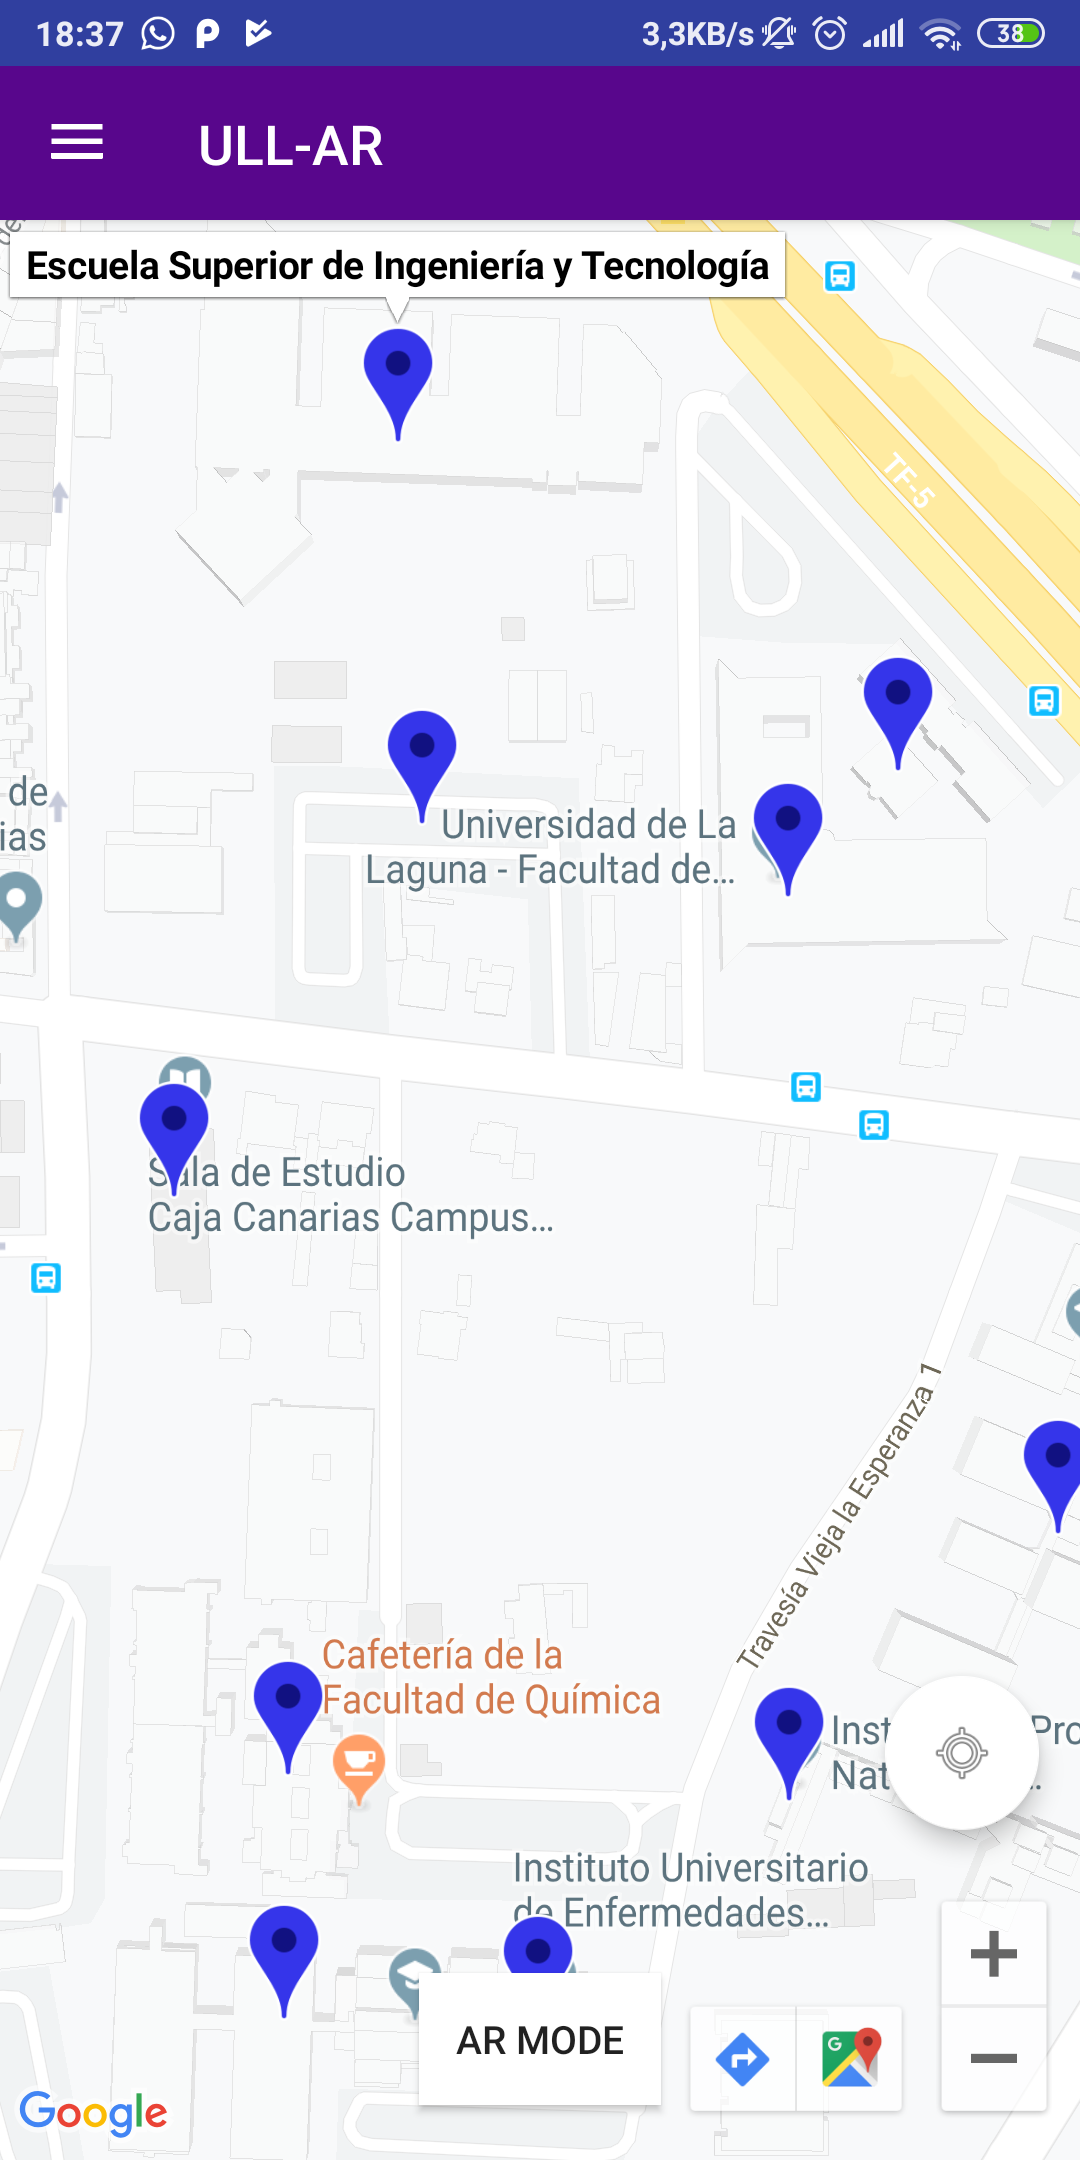
\includegraphics[width=0.38\linewidth]{mapsApp}
	\caption{Mapa ULL.}
	\label{fig:mapsApp}
\end{figure}

En la ventana de \textit{Navegación en modo RA} se nos mostrará la cámara XXX


% \begin{figure}[h]
%     \hspace*{\fill}%
%     \begin{subfigure}[h]{0.35\linewidth}
%     \includegraphics[width=\linewidth]{App}
%     \caption{Ventana de \textit{Inicio}}
%     \label{fig:homeApp}
%     \end{subfigure}
%     \hfill%
%     \begin{subfigure}[h]{0.35\linewidth}
%     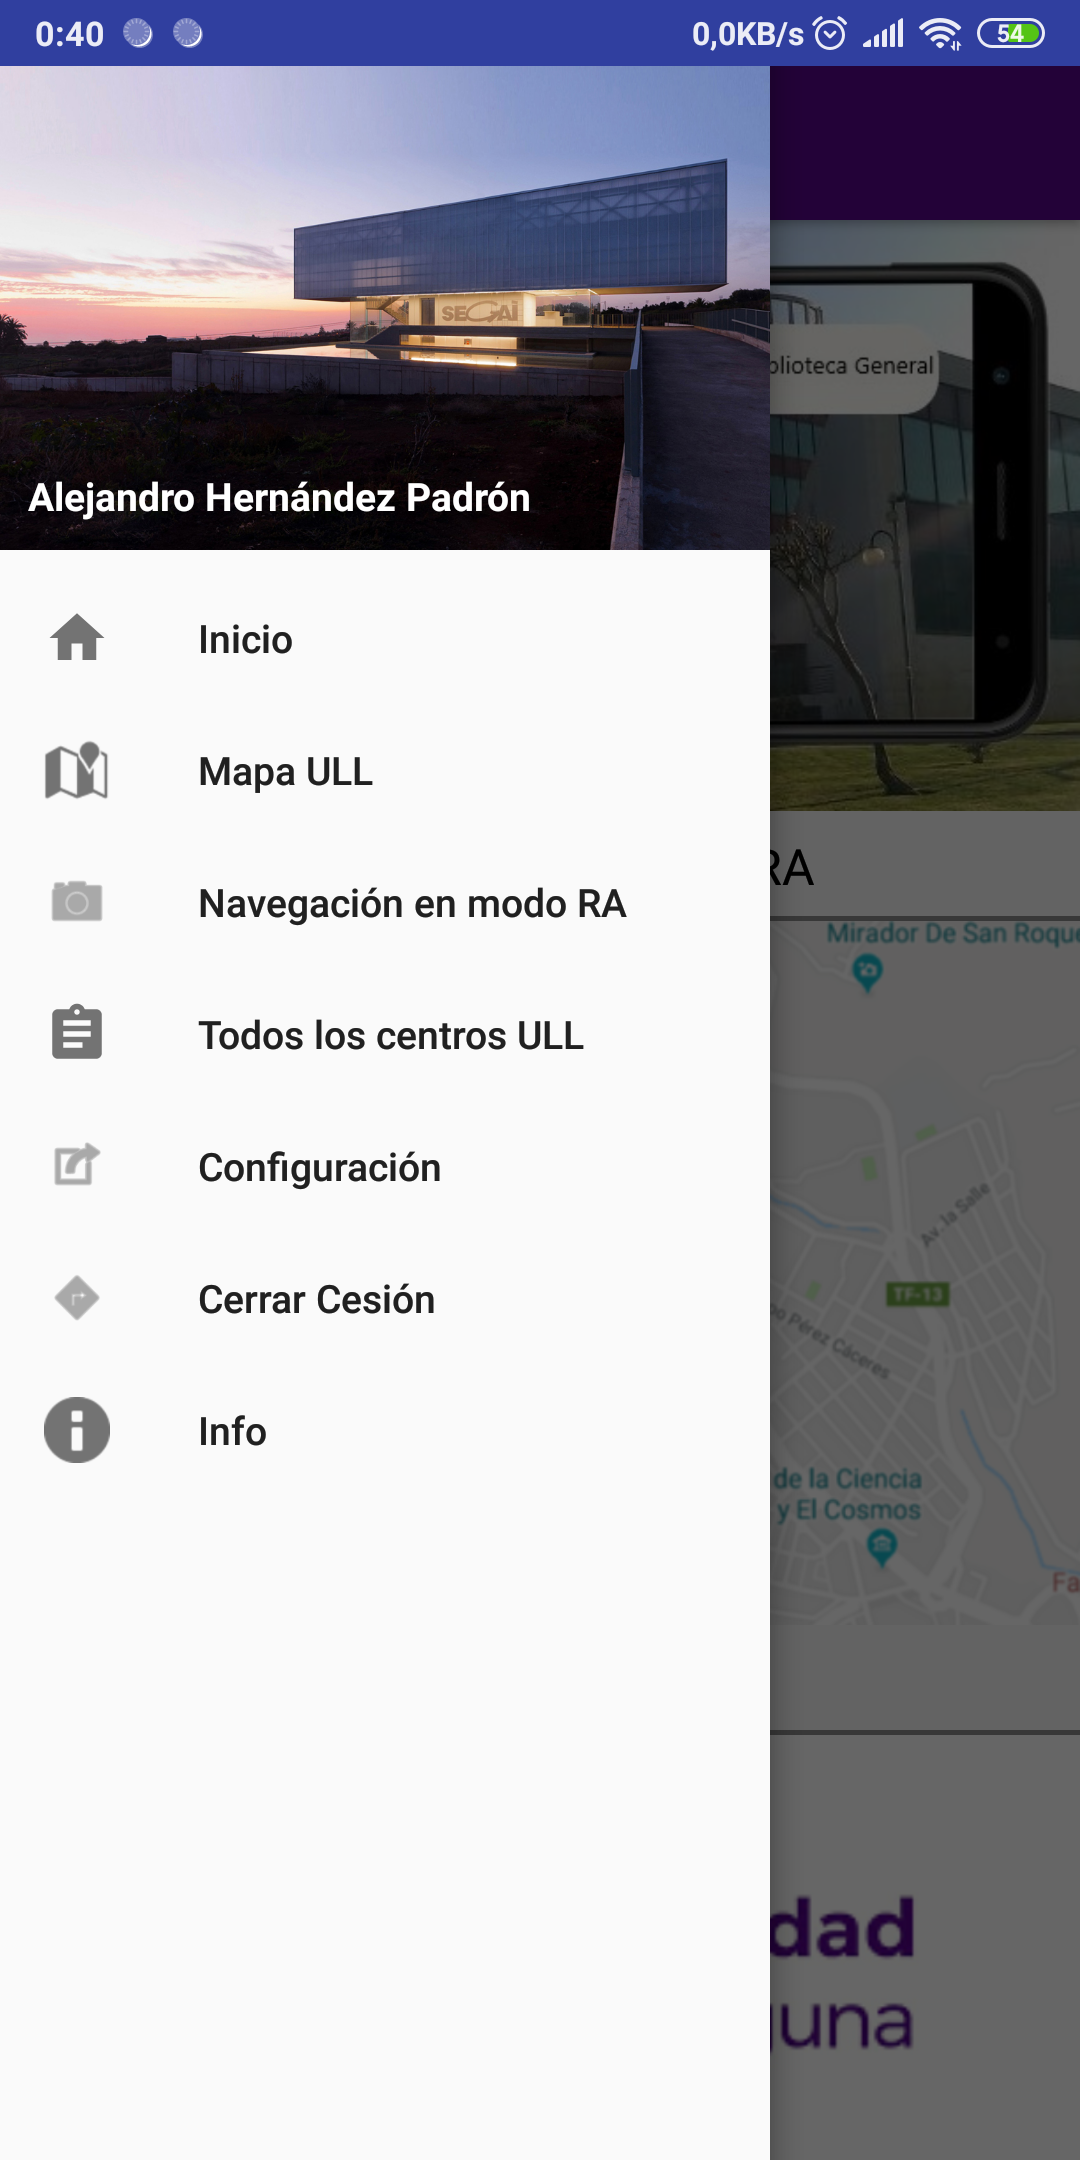
\includegraphics[width=\linewidth]{menuApp}
%     \caption{Ventana de \textit{Inicio}}
%     \label{fig:menuApp}
%     \end{subfigure}%
%     \caption{Ventana Inicio y menu de \textit{ULL-Navigation}}
%     \hspace*{\fill}%
% \end{figure}


A través del menú de la aplicación podemos acceder a la ventana de \textit{Todos los centros ULL} (vease Figura \ref{fig:allSitesApp}). Aquí se nos mostrarán todos los centros de la ULL que se encuentran en la base de datos. Se podrá hacer un búsqueda de cualquier centro en la barra superior de la aplicación. Si pulsamos cualquiera de estos centros se nos desplegará una ventana con la información detallada del centro.

En esta ventana (vease Figura \ref{fig:siteInfoApp}) se mostrará la información referente al centro. Aquí se nos mostrará una imagen del mismo, nombre y descripción del centro y una lista de enlaces con los servicios, secretarias, grados y departamentos que podemos encontrar. Disponemos de un botón en la parte inferior de la imagen del centro que nos abrirá la ruta a la ubicación del centro en Google Maps para poder llegar a él.  
 
\begin{figure}[h]
    \hspace*{\fill}%
    \begin{subfigure}[h]{0.35\linewidth}
    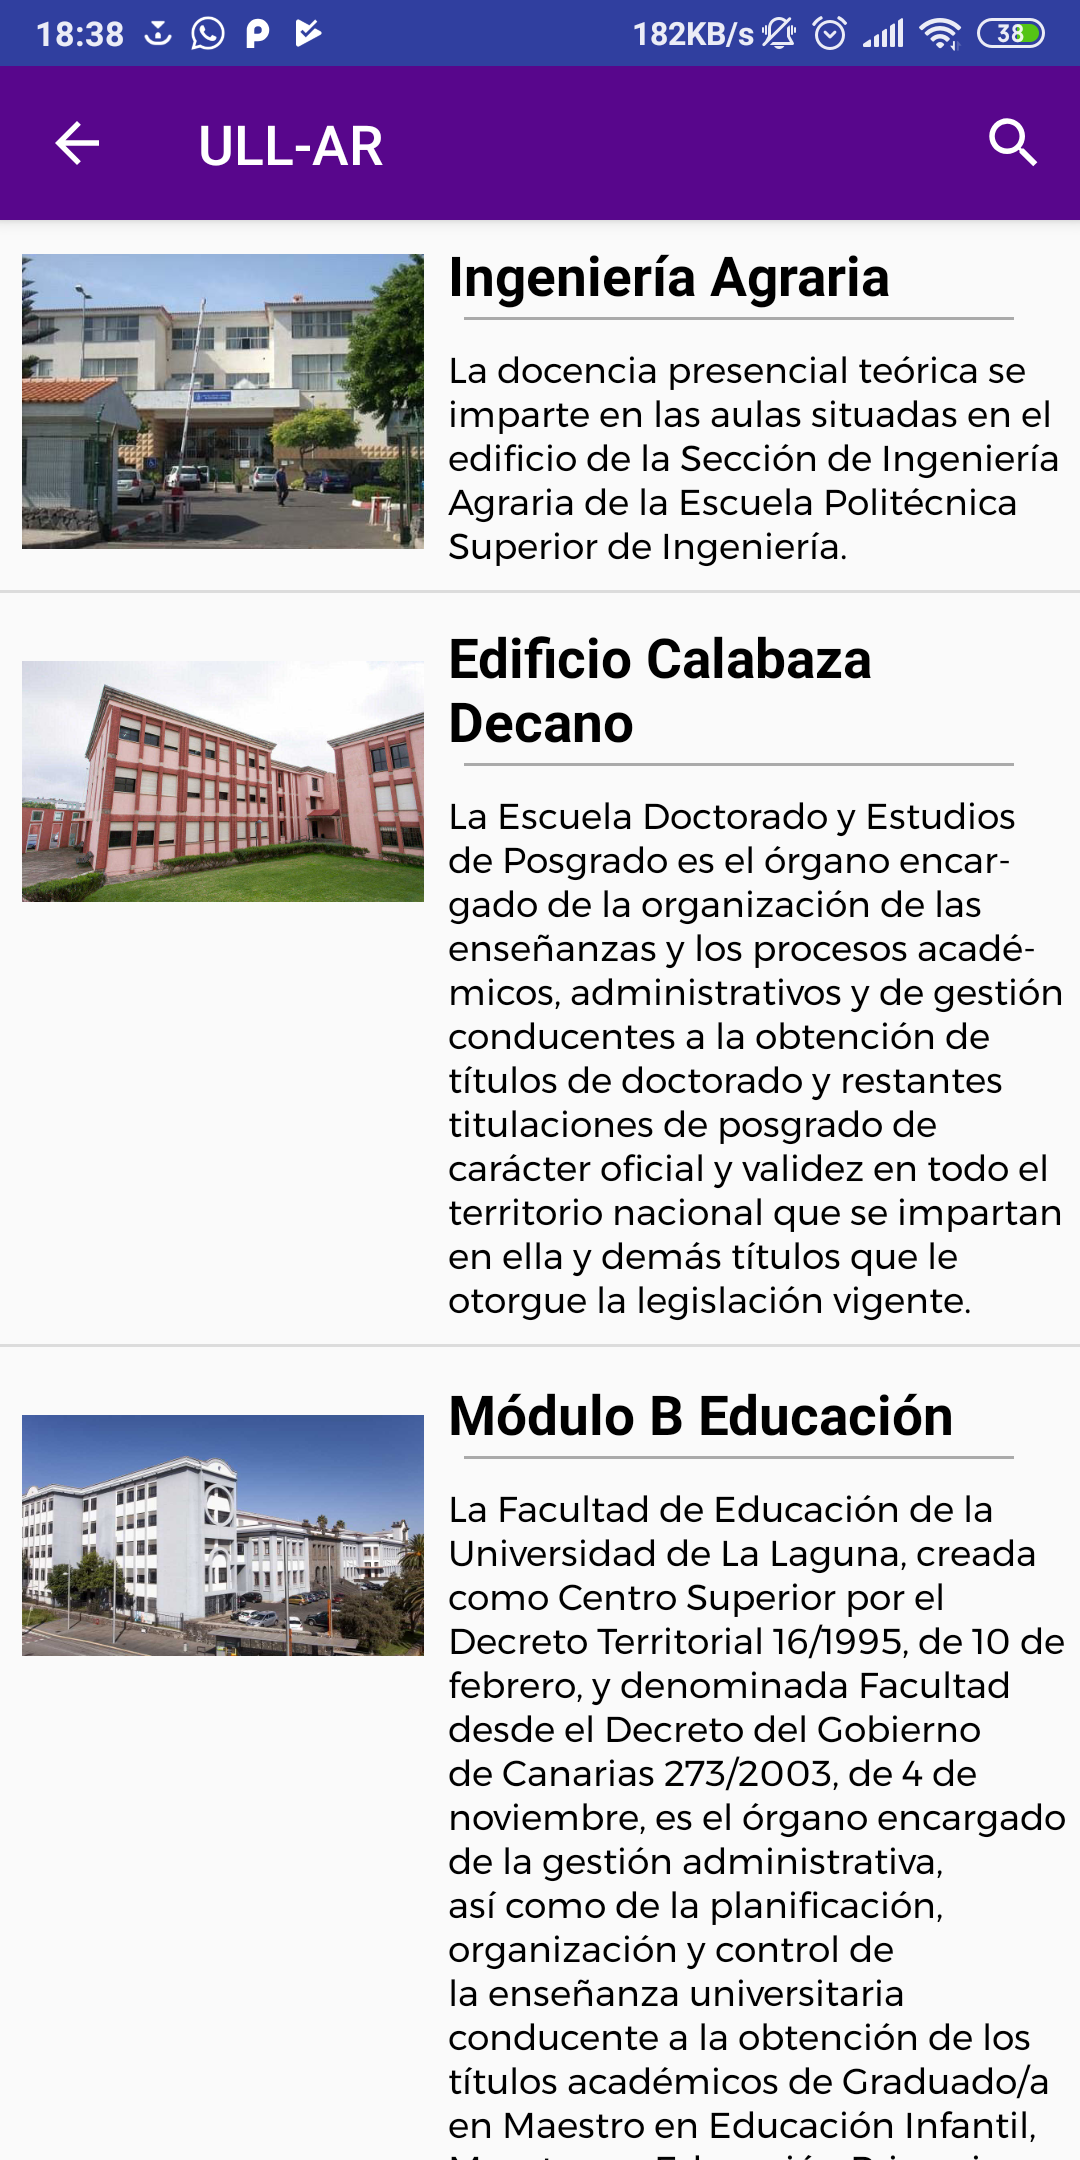
\includegraphics[width=\linewidth]{allSitesApp}
    \caption{Todos los centros ULL.}
    \label{fig:allSitesApp}
    \end{subfigure}
    \hfill%
    \begin{subfigure}[h]{0.35\linewidth}
    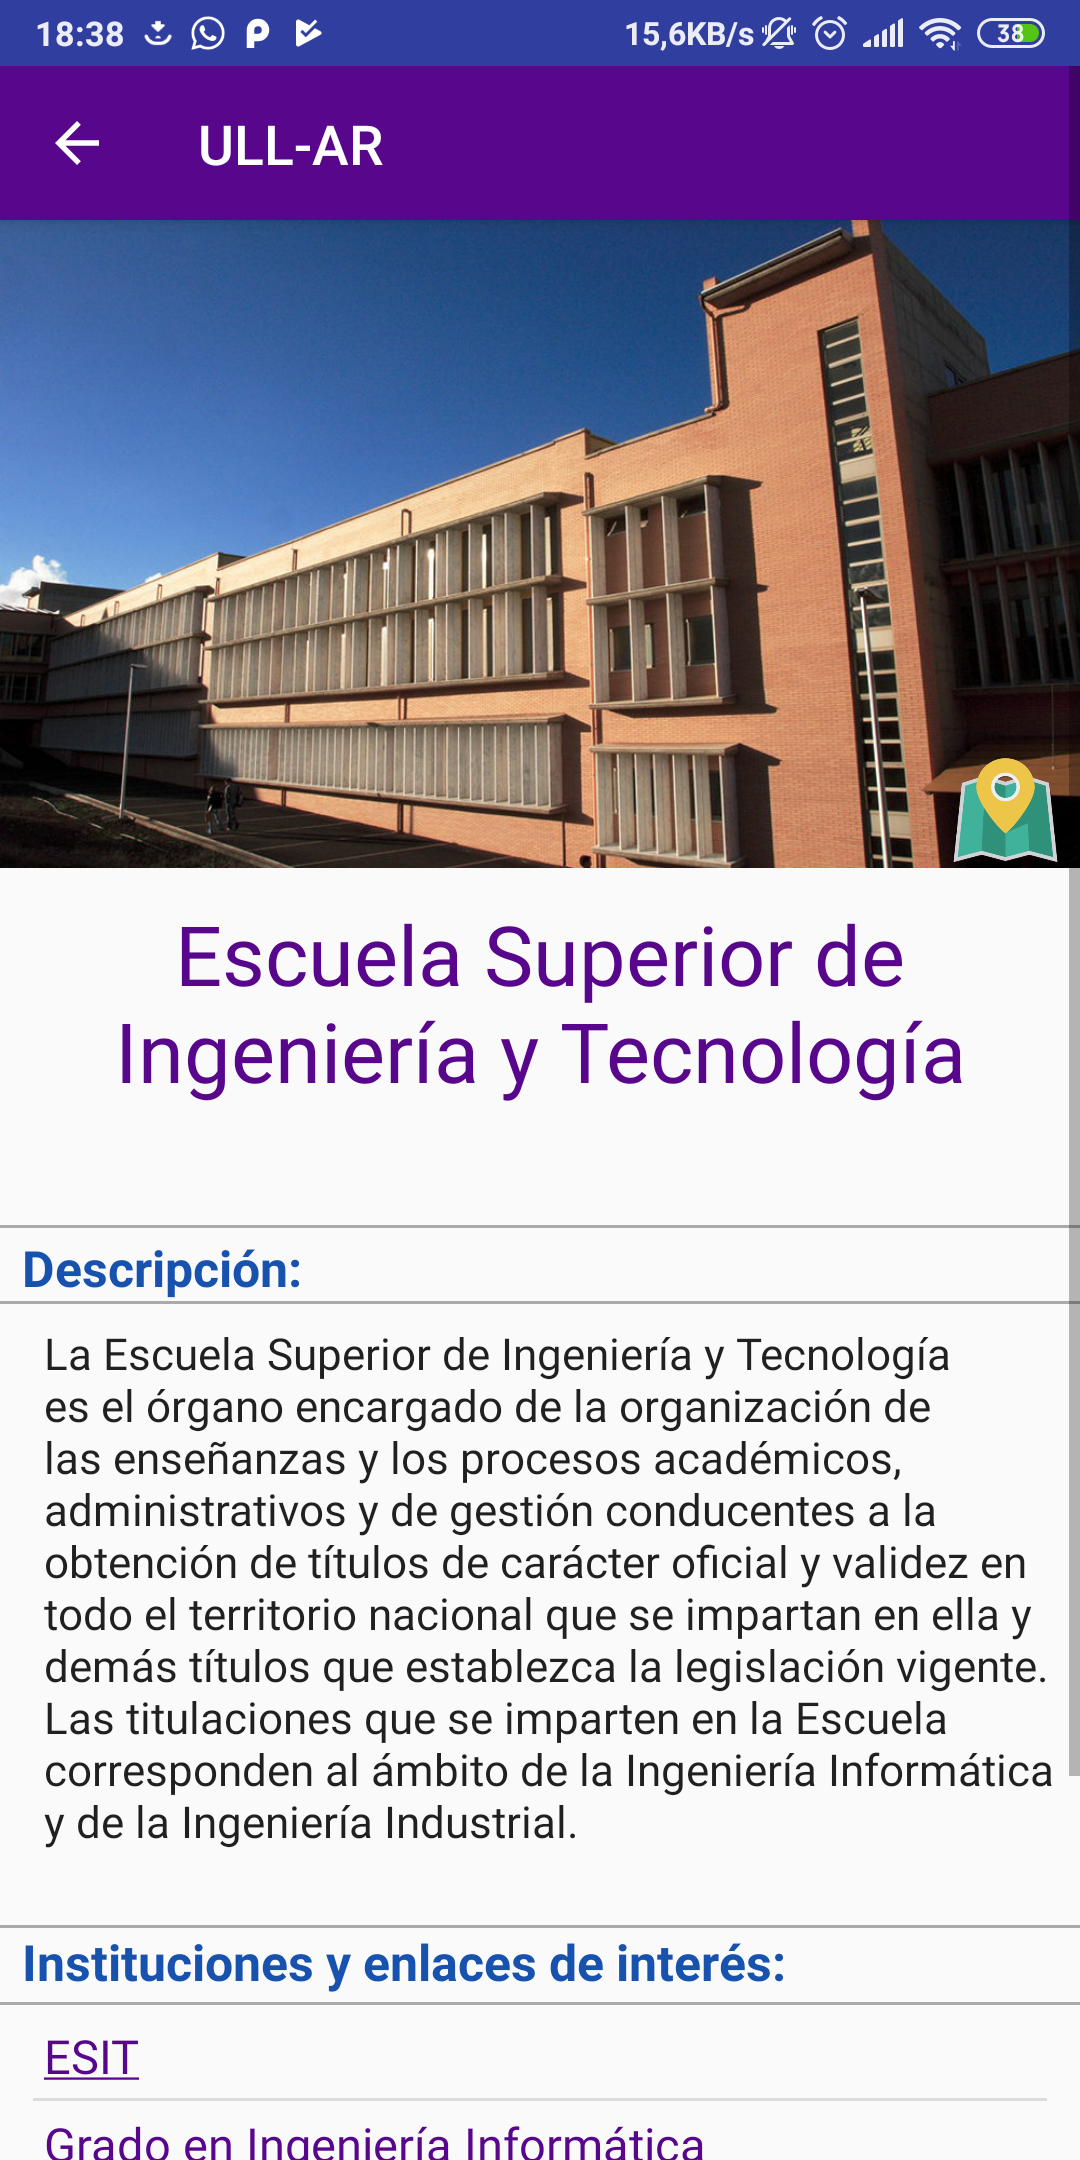
\includegraphics[width=\linewidth]{siteInfoApp}
    \caption{Información del centro.}
    \label{fig:siteInfoApp}
    \end{subfigure}%
    \caption{Ventanas de \textit{Todo los centros ULL} e \textit{Información del centro} de \textit{ULL-Navigation}.}
    \hspace*{\fill}%
\end{figure}
 

\vskip 0.9in

Por último desde el menú podemos acceder a las ventanas de \textit{Configuración} y \textit{Información}.

En la ventana de \textit{Configuración}(vease Figura \ref{fig:settingsApp}) van los ajustes de la aplicación. En la ventana tenemos la opción para poder configurar si queremos encontrar los centros que se encuentran en el área entre dos circunferencias.

La ventana \textit{Información} (vease Figura \ref{fig:infoApp}) nos muestra información básica de la aplicación como el nombre, versión, correo de contacto, autor y objetivo e información de la app \textit{ULL-Navigation}. 

\begin{figure}[h]
    \hspace*{\fill}%
    \begin{subfigure}[h]{0.35\linewidth}
    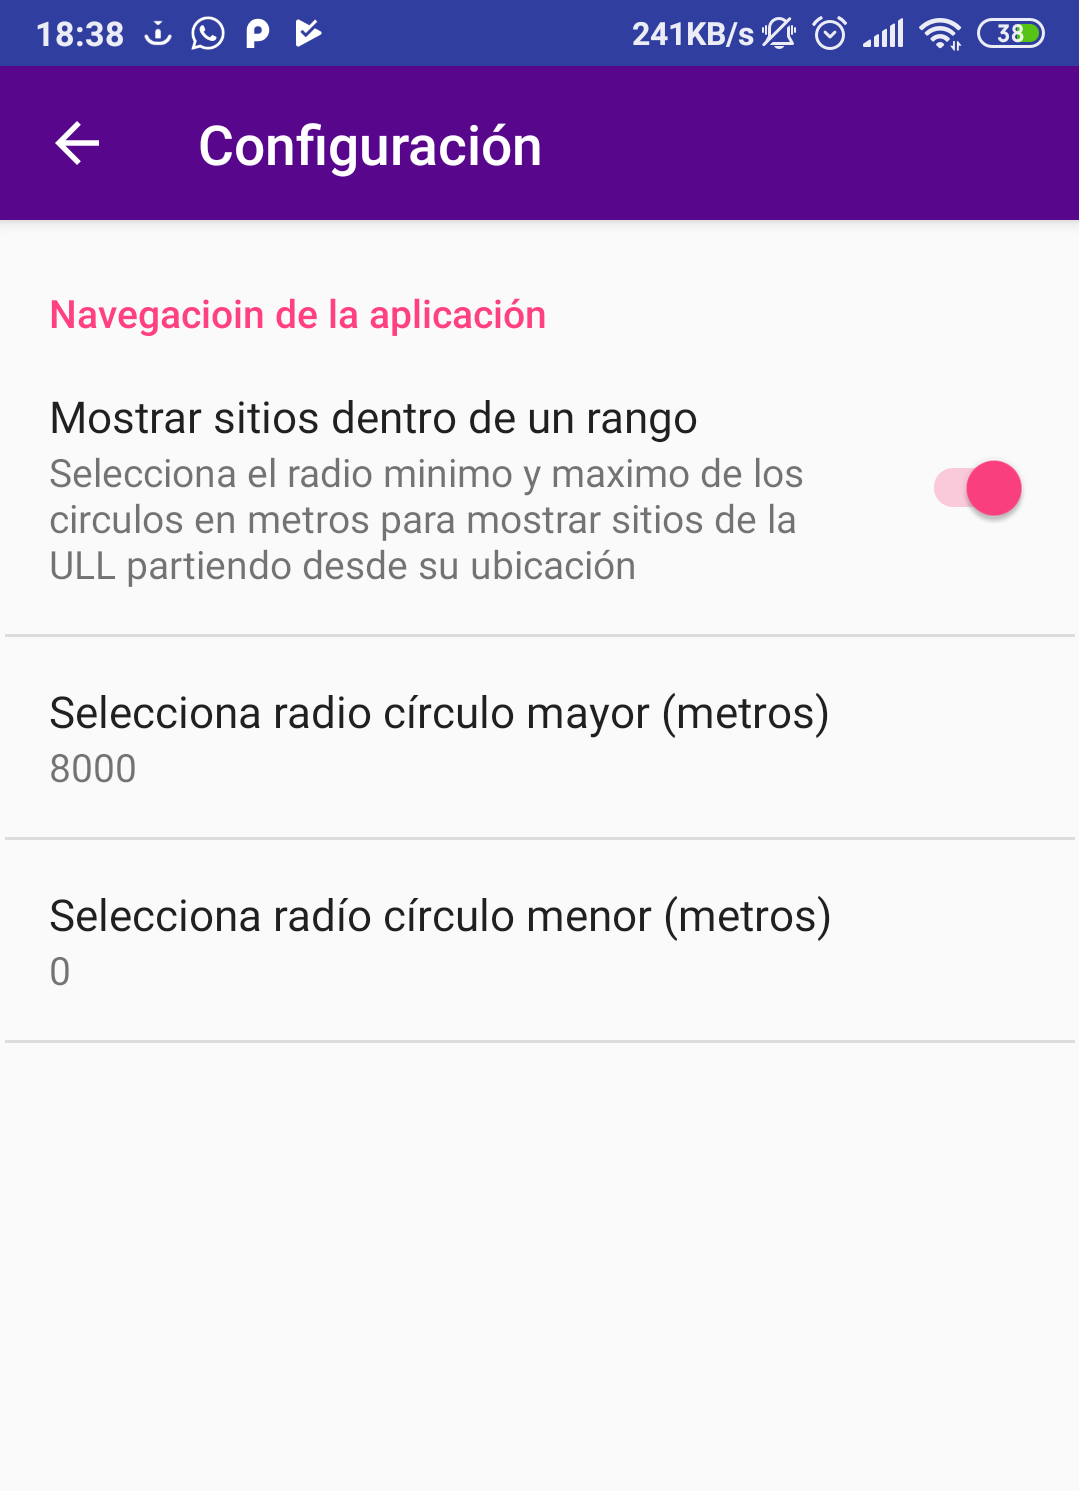
\includegraphics[width=\linewidth]{settingsApp}
    \caption{Configuración.}
    \label{fig:settingsApp}
    \end{subfigure}
    \hfill%
    \begin{subfigure}[h]{0.35\linewidth}
    
\includegraphics[width=\linewidth]{infoApp}
    \caption{Información.}
    \label{fig:infoApp}
    \end{subfigure}%
    \caption{Ventanas de \textit{Configuración} e \textit{Información} de \textit{ULL-Navigation}.}
    \hspace*{\fill}%
\end{figure}


% subsection  (end)

% -El tfg se realizara en latex
% -Desarrollo en linux
% -Movernos por la universidad
% -Realidad aumentada estudio
% -AR sdk para android 
% -AR por locacizacion
% -Maps
% -Todos los centros universitarios con su locacizacion nombre, descripcion y enlaces de las instituciones.
% -Splash screen
% -Autentificacion con cuenta google de a ULL
% -Ficha de los sitios
% -Posibilidad de cerrar sesion 
% -Pestaña de informacion de la aplicacion
% -Una pestaña de configuracion 
% -Back-end, servidor y base de datos en la nube para mayor facilidad en las pruebas 
% -




% \section{Implementación}
% \section{Desarrollo}











% \lstset{numbers=left, stepnumber=2, frame=single,}
% \lstinputlisting[float, floatplacement=H, caption={La clase \textit{Arrival} donde quedan contenidos los datos de cada llegada.}, label={code:arrival}]
% {listings/Arrival.java} %% LISTING
